\begin{center}
\fbox{\fbox{\parbox{6.5in}{\centering
PÖÖRDVÕRDELINE SÕLTUVUS. PÖÖRDVÕRDELISE SÕLTUVUSE GRAAFIK.\\
\begin{flushleft}
\hspace{5mm}
\textbf{Pöördvõrdeline sõltuvus}\\
\vspace{5mm}
\hspace{5mm}
Pöördvõrdelise sõltuvuse puhul, on $y$ väärtused pöördvõrdelises seoses $x$-idega.\\
\hspace{5mm}
See tähendab, et $x$-i suurenemisel, muutuvad $y$ väärtused väiksemaks.\\
\hspace{5mm}
Pöördvõrdelise seose funktsiooni võib üldisel kujul kirja panna nõnda:\\
\vspace{2mm}
\hspace{5mm} \boxed{$y=\dfrac{a}{x}$}\\
\vspace{2mm}
\hspace{5mm}
Uurime näiteks pöördvõrdelist funktsiooni $y=\dfrac{4}{x}$.\\
\vspace{2mm}
\hspace{5mm}
Kui lineaarse funktsiooni korral piisas meil vaid kahest $x$-i valikust, siis etteruttavalt võiks mainida, et\\ \hspace{5mm} pöördvõrdelise funktsiooni korral meil sirget ei teki, mille tõttu tasuks võtta rohkem $x$-e.\\
\hspace{5mm}
Valime $x$-ideks näiteks järgmised arvud:\\
\vspace{2mm}
\hspace{5mm}
\begin{tabular}{c|c|c|c|c|c|c|c|c|c|c}
     x & -10 & -5 & -2 & -1 & -0.5 & 0.5 & 1 & 2 & 5 & 10 \\
     \hline
     y &  & & & & & & & & &
\end{tabular}\\
\vspace{2mm}
\hspace{5mm} Nüüd tuleb meil valitud $x$-id asetada ükshaaval meie funktsiooni $y=\dfrac{4}{x}$ ning arvutada iga $x$-ile\\ \hspace{5mm} vastav $y$ väärtus. Pärast arvutamist peaksime saama järgmise väärtustetabeli:\\
\vspace{2mm}
\hspace{5mm}
\begin{tabular}{c|c|c|c|c|c|c|c|c|c|c}
     x & -10 & -5 & -2 & -1 & -0.5 & 0.5 & 1 & 2 & 5 & 10 \\
     \hline
     y & -0.4 & -0.8 & -2 & -4 & -8 & 8 & 4 & 2 & 0.8 & 0.4
\end{tabular}\\
\vspace{2mm}
\hspace{5mm}
Nüüd võtame ükshaaval x ja y paarid ja kanname need punktidena graafikule (joonis \ref{pöördvõrd}).\\
\hspace{5mm} Meenutan, et $x$ määrab ära, mittu sammu me $0$-st paremale või vasakule tegema peame. Kui x on\\ \hspace{5mm} negatiivne, siis liigume vasakule ja kui x on positiivne, siis liigume paremale. Seejärel, kui oleme oma\\ \hspace{5mm} sammud $x$-iga ära teinud, siis liigume sealt asukohast nii palju ülesse või alla, kui palju meil $y$ ütleb.\\ \hspace{5mm} Kui $y$ on positiivne, siis liigume ülesse ja kui $y$ on negatiivne siis liigume alla. Siis märgime punkti ära\\ \hspace{5mm} ja alustame otsast peale uue x-y paariga.\\
\vspace{2mm}
\hspace{5mm} Meie näite puhul peaks graafik lõpuks välja nägema nõnda:\\
\begin{center}
    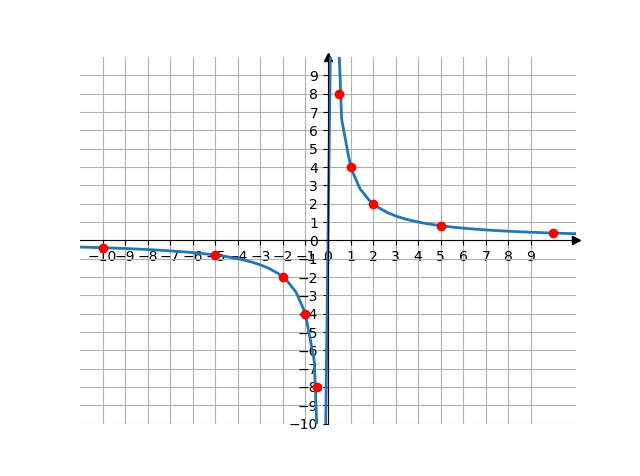
\includegraphics[width=9cm]{pöördvõrdeline.png}
    \captionof{figure}{$y=\dfrac{4}{x}$}
    \label{pöördvõrd}
\end{center}\\
\vspace{5mm}
\hspace{5mm}
Tabelist ja graafikust on näha, et tõepoolest, kui meie $x$ väärtused on väga suured (negatiivses või\\ \hspace{5mm} positiivses mõttes), siis on $y$ väärtused väga väikesed (samuti negatiivses või positiivses mõttes). Ning\\ \hspace{5mm} omakorda, kui $x$-id lähenevad nullile (muutuvad väiksemaks), siis läheb $y$ õudsalt suureks.\\
\hspace{5mm} Kuid üks oluline erinevus on selles, et üks ''suur $y$'' on negatiivse väärtusega ning teine ''suur $y$'' on\\ \hspace{5mm} positiivse väärtusega. ''Suure'' all mõeldakse siin pigem $y$ absoluutväärtust.

\end{flushleft} 
}}}
\end{center}